\chapter{Large-Scale Entity Representation}
\label{sec:EntityRepresentation}

The true power of a Data-Oriented simulation is often measured by its visual density, the ability to render thousands of individual agents without compromising the frame rate or visual fidelity. However, as the entity count scales up, the primary bottleneck shifts from CPU logic to GPU throughput and draw calls.

In traditional game developement, the visual presence of an object is inextricably linked to its logical container, in Unreal Engine this container is typically the \texttt{AActor}. In the Mass Framework this link is severed. Mass Representation serves as the managing layer that translates abstract entity data into high-performance visual primitives, primarily batching thousands of individual entity transforms into a single Instanced Static Mesh draw call.

This chapter explores this architectural shift by treating representation as a dynamic state rather than a static component property. We begin by diagnosing the inherent limitations of the Actor-centric model, specifically analyzing how \texttt{UObject} overhead and individual draw calls create a performance ceiling that traditional architectures cannot breach.

Once these bottlenecks are established, the discourse moves to the Mass LOD system, which serves as the simulation’s brain for visibility and performance throttling, orchestrating agent fidelity based on spatial relevance. This leads into a technical examination of standard representation strategies, where we analyze the mechanics of Instanced Static Meshes (ISM) and the AnimToTexture pipeline, the dual frameworks that enable high-fidelity crowd visualization at scale. Finally, we explore alternative and non-standard approaches, such as Niagara-based representation and hybrid solutions.


% use [] to set name for ToC
\section[Actor-based Representation Limitations]{Actor-based Representation Limitations} % ok with fontsize=12pt

In the standard Unreal Engine workflow, the \texttt{AActor} serves as a monolithic container that inextricably links an object's logical state with its visual presence. While this is ideal for individual player characters, it introduces some critical bottlenecks when scaling to thousands of agents.

The \texttt{UObject} system comes with a computational overhead: each actor requires dedicated memory for reflection metadata, property tracking and integration with the garbage collection system. Simply maintaining the memory footprint of thousands empty actors can saturate the system resources even before simulation logic is processed. 

\begin{figure}[h]
\centering
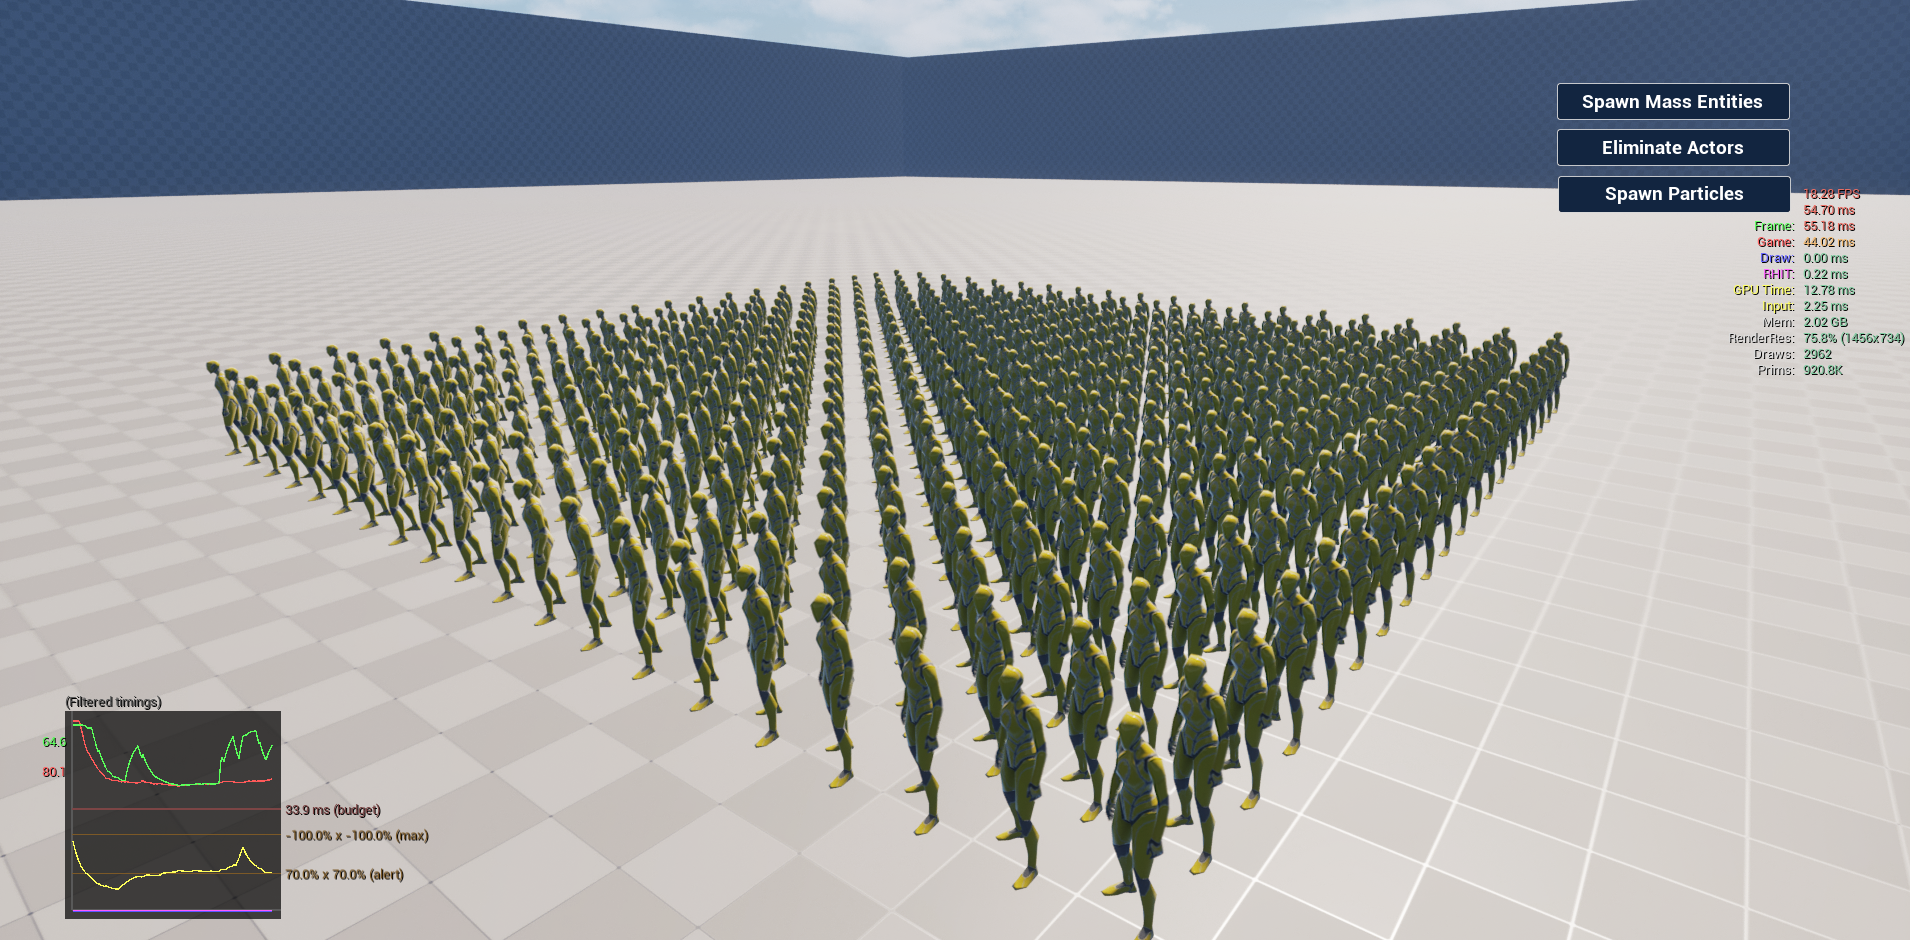
\includegraphics[width=1\textwidth]{images/ActorPerformanceFPSGrid.png}
\caption{CPU performance tanking when a grid of actors is instanced in an empty scene. The Game Thread took 44ms to process this frame, hence lowering the FPS.}
\end{figure}

This overhead extends into the rendering pipeline, creating a draw call ceiling. Because each Actor’s \texttt{UStaticMeshComponent} typically generates its own unique render commands, the CPU's command buffer becomes a critical bottleneck. The CPU spends so much time preparing and submitting tens of thousands of individual instructions that it cannot keep pace with the GPU, leaving the graphics hardware idle while the CPU-side rendering thread is saturated.

% aggiungi immagine insights con questo fatto delle draw call che si vede (stalli GPU)

Finally, the architecture suffers from sequential scene updates driven by the hierarchical \texttt{USceneComponent} system. Every frame, the engine must recursively calculate world-space transforms, update bounding volumes, and perform individual visibility culling checks for every agent on the Game Thread. When the number of entities scales, this transform overhead alone can exceed the entire 16.6ms per frame budget, making real-time performance impossible within the traditional Actor-centric paradigm.

\subsection[The Mass Solution]{The Mass Solution}

Mass Representation addresses the limitations of the Actor model by severing the link between an entity’s logical existence and its visual manifestation. In this paradigm, the entity remains a lean data construct, while its physical presence in the world is managed by a dedicated translation layer. This architectural shift replaces the static one-to-one relationship of Actors with a dynamic visual proxy system, where the method of rendering is merely a transient state determined by the entity's current relevance to the observer.

The efficiency of this solution is rooted in the way the Mass Representation Processor interacts with the entity’s existing spatial data. Instead of each agent being responsible for its own rendering, the processor iterates over the \texttt{FTransformFragment} data in a high-performance, cache-aligned stream. This allows the system to gather the transforms of thousands of entities simultaneously and push them into a centralized rendering backend.

The primary tool for this large-scale visualization is the Instanced Static Mesh (ISM), or more specifically, the Hierarchical Instanced Static Mesh (HISM). By batching these gathered transforms into a single component, Mass collapses what would traditionally be thousands of individual draw calls into a handful of GPU-optimized operations. This is critical because every draw call represents a significant communication overhead from the CPU to the GPU. In a non-instanced scenario 30000 entities, each with a mesh and unique material attributes, would generate upwards of 60000 draw calls, overwhelming the CPU’s command buffer and leading to a complete collapse in frame rate.

Through the Mass Representation Subsystem, these entities are not merely rendered, but managed through a transactional phase. Instead of individual updates, the system pushes contiguous arrays of transforms and Per-Instance Custom Data (PICD), such as animation indices or color variations, to the GPU buffers in a single, streamlined operation. This system does not apply a uniform representation to all entities; instead, it utilizes a multi-tiered Level of Detail (LOD) logic to determine whether an entity should be rendered as a high-fidelity Actor, a high-performance HISM instance, or culled entirely based on its spatial relevance to the viewer.

\section[Mass Level Of Detail]{Mass Level Of Detail}

The Mass LOD system serves as the central decision-making engine for entity relevance. Unlike traditional LOD systems that only swap mesh resolutions, Mass uses LOD to drive a multi-system load balancing strategy. By categorizing entities into four distinct states (High, Medium, Low, and Off) the framework can dynamically throttle everything from rendering fidelity to the frequency of C++ logic updates.

\subsection{Mass LOD Overview}

The LOD Subsystem does not act alone, it serves three primary clients that use its spatial calculations to optimize different hardware bottlenecks:

\begin{itemize}
    \item \textbf{Mass Visualization LOD}: manages the visual proxy swapping discussed in the previous section. It determines if an entity should be an Actor, an ISM, or culled entirely based on distance and camera frustum visibility
    \item \textbf{Mass Simulation LOD}: implements time throttling and variable ticking. It allows the CPU to skip update frames for distant entities. For example, we could be updating a distant agent’s logic 5 times per second instead of 60.
    \item \textbf{Mass Replication LOD}: optimizes network bandwidth by reducing the frequency of data synchronization for entities far from the player
\end{itemize}

\subsection{Mass LOD Subsystem}

The \texttt{UMassLODSubsystem} acts as the global state provider for spatial relevance, serving as the synchronization point between the Game Thread's camera data and the Mass ECS simulation. In a high-density simulation, having tens of thousands of entities independently query the \texttt{APlayerController} for camera coordinates would create a relevant CPU bottleneck. The subsystem solves this by centralizing viewer management, ensuring that the heavy lifting of gathering engine-side world state is performed only once per frame.

Technically, the subsystem is hooked into the \texttt{PrePhysics} phase of the \newline\texttt{UMassSimulationSubsystem}. At the start of this phase, it iterates through all active controllers, camera components, and World Partition streaming sources to populate a internal temporary array of \texttt{FViewerInfo} structures. Each entry in this array serves as a lightweight snapshot of an observer's perspective, encapsulating the following properties: 

\begin{itemize}
    \item \textbf{Location and Rotation}: he world-space origin and orientation of the viewer
    \item \textbf{Field of View (FOV) and Aspect Ratio}: critical parameters used to derive the frustum planes for visibility culling
\end{itemize}

This centralized array acts as the source of truth for all downstream LOD clients. Rather than entities pulling data from the world, the \newline\texttt{UMassLODCollectorProcessor} pushes the subsystem's cached viewer data into the entity fragments. To determine how an entity archetype should interact with this viewer data, Mass provides two primary collector traits that define the policy for relevance calculation:

\begin{itemize}
    \item \texttt{UMassDistanceLODCollectorTrait}: this trait is the more computationally lean of the two. It adds the \texttt{FMassCollectDistanceLODViewerInfoTag}, triggering the \texttt{UMassLODDistanceCollectorProcessor}. This processor calculates relevance based purely on radial proximity to the nearest viewer, ignoring the viewer's orientation. This is ideal for systemic logic, such as background AI, that must remain active even if the agent is behind the camera.
    \item \texttt{UMassLODCollectorTrait}: the standard collector trait adds the \newline\texttt{FMassCollectLODViewerInfoTag}, triggering the \newline\texttt{UMassLODCollectorProcessor}. This version utilizes the full frustum data provided by the subsystem to perform a dot-product based visibility test. It is the primary choice for visualization, allowing the system to demote entities to an Off state the moment they exit the camera's view.
\end{itemize}

%add image of the traits added in the editor (?) OR image of the difference (è difficile da fare perchè non si vede tanto)

% manca una parte dove parlo dei tag che esistono per i vari livelli di LOD e come usarli per filtrare le entità e una parte dove parlo degli if che si possono usare per applicare comportamenti diversi a livelli di lod diversi nello stesso processore

Rather than entities pulling data from the world, these processors push the subsystem's cached viewer data into the entity fragments. This is facilitated by the \texttt{TMassLODCollector} processor, which performs high-speed comparisons between the global \texttt{FViewerInfo} array and the local \texttt{FTransformFragment} of each entity.

The output of this process is the population of the \texttt{FMassViewerInfoFragment}. By storing the \texttt{ClosestViewerDistanceSq} and \texttt{ClosestDistanceToFrustum} directly on the entity, Mass allows other systems, such as the Simulation and Representation processors, to perform constant-time checks on an entity's relevance. This architecture effectively decouples the complexity of the world’s viewing conditions from the per-entity logic, ensuring that even with a large number of agents, the overhead of determining visibility remains a linear, cache-friendly operation.

\section{Mass Representation}

The \texttt{UMassRepresentationProcessor} is the execution engine that synchronizes an entity’s logical state with its visual manifestation. It operates by evaluating the results stored in the \texttt{FMassViewerInfoFragment} and the current LOD tags to determine the appropriate \texttt{EMassRepresentationType}. This enum acts as a state machine for the entity's visual proxy, supporting four primary modes:

\begin{itemize}
    \item \textbf{HighResSpawnedActor}: the entity is represented by a full, high-fidelity \texttt{AActor}. This is reserved for the highest LOD (typically \texttt{EMassLOD::High}), enabling complex skeletal mesh animations, physics interactions, and full component functionality.
    \item \textbf{LowResSpawnedActor}: a lightweight version of the Actor representation. This is often used for entities that are visible but not in the immediate foreground. It may swap the complex skeletal mesh for a simpler one or disable expensive components, such as complex AI or ticking components, while maintaining the \texttt{AActor} wrapper for basic interaction or sound.
    \item \textbf{StaticMeshInstance}: the entity is rendered via the HISM (Hierarchical Instanced Static Mesh) system. This is the ideal representation for performance, allowing thousands of agents to be drawn in a few GPU batches. In this state, the entity no longer exists as an \texttt{AActor} in the world; it is merely a transform and a set of custom data in a GPU buffer.
    \item \textbf{None}: The entity is completely culled. The mesh is removed from the render pipeline entirely, though the underlying Mass simulation continues to run.
\end{itemize}

The transition between these states is managed through the \newline\texttt{FMassRepresentationFragment}, which tracks both the \texttt{CurrentRepresentation} and \texttt{PrevRepresentation}. This allows the system to handle the "setup and teardown" of visual assets, such as calling the \texttt{UMassActorSpawnerSubsystem} to spawn an Actor or clearing an index from a HISM, only when a state change occurs, preventing expensive per-frame logic.

\subsection{Vertex Animated ISM}

For large crowds of entities, traditional skeletal mesh skinning (calculating bone offsets on the CPU) is a primary bottleneck. A way to bypass this is found by leveraging AnimToTexture (Vertex Animation Texture).

In this workflow, animation data is baked into a 2D HDR texture where rows represent bones and columns represent time frames. During the \texttt{StaticMeshInstance} representation phase, the HISM vertex shader samples this texture to offset vertices directly on the GPU. This transforms the computational cost of an animated character into that of a static mesh with a specialized material. To ensure the crowd does not appear synchronized, it is possible to push Per-Instance Custom Data (PICD) via Mass to the HISM. In the standard AnimToTexture shader at scale, the two critical floats are typically: 

\begin{itemize}
    \item \textbf{Animation State / Index}: This tells the shader which row of the baked texture to read, allowing to select the animation among the baked ones. This is often a quantized float derived from the \texttt{FMassCrowdAnimationFragment}.
    \item \textbf{Normalized Animation Phase}: Instead of a global time offset, Mass frequently calculates and pushes the actual playback position (as a value going from 0.0 to 1.0) of the animation loop. This is calculated on the CPU by taking the entity's internal clock, adding a random seed, and modulo-ing it by the animation duration.
\end{itemize}

The practical application of this vertex-driven animation pipeline is most notably demonstrated in Unreal Engine’s City Sample project, where the \newline\texttt{UMassCrowdAnimationProcessor} serves as a specialized extension of the core Mass framework to orchestrate the movement of thousands of simulated pedestrians.

%aggiungere spiegazione su possibili ottimizzazioni delle animazioni per i normali actor?

\section{Niagara Representation}

% non sono super certa che abbia senso parlare di questa cosa, perchè è molto complessa. Vedere come la fanno in mass sample e decidere